 
  \documentclass{article} 
  \usepackage{amsmath} 
  \usepackage{graphicx} 
  \usepackage{float} 
  \usepackage{listings} 
  \lstset{language=Matlab,basicstyle=\ttfamily,commentstyle=\ttfamily} 
  \title{\textsf{MatLaTex}: Embedding \textsf{Matlab} Results in \LaTeX\ Documents\\ {\small version 2022.02.05}} 
  \author{Athanasios Kehagias\\kehagiat@ece.auth.gr} 
  \setlength{\textwidth}{6.75in} 
  \setlength{\textheight}{9.00in} 
  \setlength{\oddsidemargin}{0 in} 
  \setlength{\topmargin}{0 in} 
  \begin{document} 
  \maketitle 
  \section{Introduction} 
  \texttt{MatLaTex.m} is a \emph{very simple} script intended to enable the user to \emph{programmatically}  
  include the results of \textsf{Matlab} computations in \LaTeX\  documents; 
  the focus is on \emph{symbolic} computations but numerics and figures can also be used.  
  Hence it is similar in purpose to the various ``sweave'' packages that exist for both \textsf{Matlab}  and other 
  languages, e.g. \textsf{SageMath}, \textsf{R}, \textsf{Python} etc. But the emphasis of \textsf{MatLaTex} is on \emph{simplicity}. 
  \footnote{Further discussion of this point appears in the Postscript.} 
  
  \section{Installation} 
  Simply unzip the file \texttt{MatLatex.zip} into some folder. You must have installed \textsf{Matlab},  
  the  \textsf{Matlab Symbolic Math Toolbox} and a \TeX\  distribution.  
  I have tested \textsf{MatLatex} with \textsf{Matlab R2018b} and \textsf{TeX Live 2019}. 
  It works on \textsf{Windows 7, 10, 11}; since it only depends on \textsf{Matlab} and \LaTeX\, 
  it should also work on the \textsf{Linux} and \textsf{Apple} operating systems 
  (but I have not tested this). 
   
  \section{QuickStart} 
  In the \textsf{Matlab} environment, run the script \texttt{MatLatex.m}.  
  You will get the files \texttt{MatLatex.tex} and \texttt{MatLatex.pdf} (this document). 
  Open \texttt{MatLatex.m} to see the code which produces the results of this document 
  (the contents of \texttt{MatLatex.m} will be explained in a later section). 
   
  \section{Usage} 
  The \textsf{MatLaTex} workflow is as follows.  
  \begin{enumerate} 
  \item Write a \emph{single} \textsf{Matlab} script, e.g., \texttt{foo.m},  
  which contains both \textsf{Matlab} commands and \LaTeX\  code (embedded as comments); 
  the \LaTeX\  code can include the control words \texttt{latex (a)} and \texttt{num2str(b)} 
  where \texttt{a} and \texttt{b} are \textsf{Matlab} variables (details will be given in the following sections).      
  \item The file \texttt{foo.m} must be created in the same folder which contains \texttt{MatLatex.m}. 
  \item Change the second line of \texttt{MatLatex.m} from \texttt{fn='MatLatexDoc'} to \texttt{fn='foo'}. 
  \item Run \texttt{MatLatex.m} (i.e., type \texttt{MatLatex} in the \textsf{Matlab} command line). 
  \item When execution of \texttt{MatLatex.m} is completed you have the following files. 
  \begin{enumerate}   
  \item \texttt{foo.tex}: your \LaTeX\  code with \textsf{Matlab} results having replaced 
  the \texttt{latex (a)} and \texttt{num2str(b)} control words. 
  \item \texttt{foo.pdf}: the output of \texttt{foo.tex} as compiled by \textsf{pdflatex}. 
  \end{enumerate} 
  \end{enumerate} 
   
  \noindent To use \textsf{MatLaTex} follow the above  workflow. 
  The rules for writing \textsf{MatLaTex} files are as follows. 
  \begin{enumerate} 
  \item Each line contains either \emph{only} \textsf{Matlab} code  or \emph{only} \LaTeX\ code.  
  \item \textsf{Matlab} code is written as usual. 
  \item \LaTeX\ code is also written as usual with the following exceptions.  
  \begin{enumerate} 
  \item Every line of \LaTeX\ code is preceded by the characters \texttt{\%\%}  
  (so, as far as \textsf{Matlab} is concerned, these 
  are comment lines). 
  \item You can use the additional control word \texttt{latex (\;)} (\textbf{without} being preceded by a backslash!).  
  Every occurrence of \texttt{a} in the \LaTeX\  part of your code will be replaced  
  by the \LaTeX\  expression for \texttt{a}, 
  where it is assumed that \texttt{a} has been declared (in the \textsf{Matlab} part of your code) as a symbolic variable. 
  \item You can use the additional control word \texttt{num2str(\;)} (\textbf{without} being preceded by a backslash!). 
  Every occurrence of \texttt{num2str(a)} in the \LaTeX\ part of your code will  
  be replaced by the \texttt{num2str}  expression for  \texttt{a}, 
  where it is assumed that \texttt{a} has been declared / computed (in the \textsf{Matlab} part of your code)  
  as a $1\times 1$ double variable.  
  
  \medskip  
   
  \noindent\textbf{Nota Bene}: 
  This means that you can only use \texttt{num2str (\;)} to render \emph{scalar} doubles. If you want  
  to render a double matrix \texttt{A}, 
  you must define a symbolic variable \texttt{Z} by \texttt{B=sym(A)} and then use \texttt{latex(Z)}. This works well when  
  the entries of \texttt{A} are integers or simple fractions; but if \texttt{A} has entries with many decimals, 
  \texttt{Z}  will be represented by fractions with large integer numerators and denominators. So this  
  is an issue which I hope to fix at a later version of \textsf{MatLaTex}. 
  
  \end{enumerate}   
  \end{enumerate}   
  
  \section{Some Examples and Explanations} 
  Let us now look at some parts of \texttt{MatLatexDoc.m}. 
  \begin{enumerate} 
  \item The file starts with the lines  
  \begin{lstlisting} 
  %% \documentclass{article} 
  %% \usepackage{amsmath} 
  %% \usepackage{graphicx} 
  \end{lstlisting} 
  and continues like this with typical \LaTeX\ preamble commands. Note that, since these are  
  \LaTeX\ commands, they are preceded by \texttt{\%\%}. 
  \item After a while we have   
  \begin{lstlisting} 
  %% \begin{document} 
  %% \maketitle 
  %% \section{Introduction} 
  %% \texttt{MatLaTex.m} is a \emph{very simple} script intended to  
  %% implement \emph{literate programming} in \textsf{Matlab}.  
  \end{lstlisting} 
  and so on, where we write our \LaTeX\ content as usual, but always using the \texttt{\%\%} line prefix. 
  \item Things get more interesting when we introduce symbolic computations. So for example the code  
  \begin{lstlisting} 
  syms x 
  syms f(x) 
  f(x)=x*exp(x); 
  F(x)=int(f,x); 
  %% Let us write the integral of \(f(x)=latex (f)\),  
  %% i.e., \( \int latex (f) dx = latex (F)\). 
  \end{lstlisting} 
  produces the following results. 
   
  \qquad Let us write the integral of \(f(x)=x\,{\mathrm{e}}^x\), i.e., \( \int x\,{\mathrm{e}}^x dx = {\mathrm{e}}^x\,\left(x-1\right)\). 
  
  Similarly,  the code 
  \begin{lstlisting} 
  syms n 
  syms g(n) 
  g(n)=1/n^2; 
  G=symsum(g,n,1,inf); 
  G0=double(G); 
  %% Let us write the sum of \(g(n)=latex (g)\), i.e.,  
  %% \(\sum_{n=1}^\infty latex (g)  = latex (G)\).  
  %% This evaluates to \( latex (G) = num2str (G0)\).  
  \end{lstlisting} 
  produces the following results. 
  
  \qquad Let us write the sum of \(g(n)=\frac{1}{n^2}\), i.e.,  
  \(\sum_{n=1}^\infty \frac{1}{n^2}  = \frac{\pi ^2}{6}\).  
  This evaluates to \( \frac{\pi ^2}{6} = 1.6449\). 
  \item We can also include plots. For example,  the following code 
  \begin{lstlisting} 
  figure(1); plot([0:0.1:4*pi],sin(2*[0:0.1:4*pi])); axis([0 4*pi -1.1 1.1]); 
  print('FIG001.pdf','-dpdf','-r600') 
  system(['pdfcrop FIG001.pdf FIG001.pdf']); 
  %% \begin{figure}[H] 
  %% \centering 
  %% 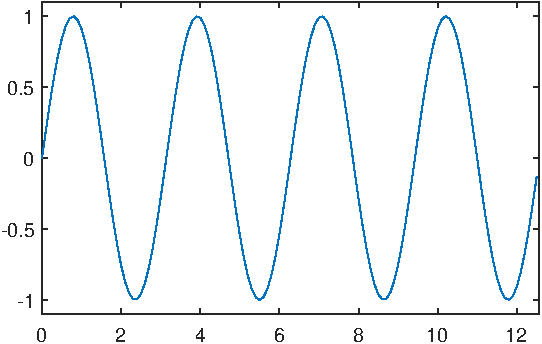
\includegraphics[scale=0.75]{FIG001} 
  %% \caption{A plot of \(f(x)=\sin(2*x)\).} 
  %% \end{figure} 
  \end{lstlisting} 
  produces the plot: 
  \begin{figure}[H] 
  \centering 
  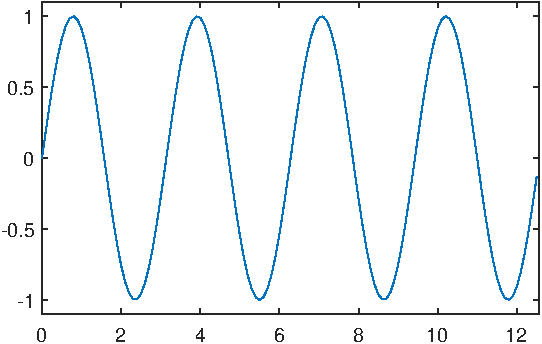
\includegraphics[scale=0.75]{FIG001.pdf} 
  \caption{A plot of \(f(x)=\sin(2*x)\).} 
  \end{figure} 
  The idea is the following. The first three lines of the above fragment  
  generate a ``regular'' \textsf{Matlab} plot, print it to file \texttt{FIG001.pdf} and then crop white space. 
  The final five lines are regular \LaTeX\ code which ``graphics -includes'' the previously produced file. 
   
  \item Let us now present  some additional symbolic results; to see the code which 
  generates the following lines open \textsf{MatLatexDoc.m} and look at around lines 180-260. 
  \begin{enumerate} 
  \item The Hessian of \(f(x,y,z)=2\,z\,x^2+x\,y^2\) is 
  \[ 
  H=\left(\begin{array}{ccc} 4\,z & 2\,y & 4\,x\\ 2\,y & 2\,x & 0\\ 4\,x & 0 & 0 \end{array}\right) 
  \] 
  \item The Jacobian of \(f(x,y,z)=2\,z\,x^2+x\,y^2\) is 
  \[ 
  J=\left(\begin{array}{ccc} y^2+4\,x\,z & 2\,x\,y & 2\,x^2 \end{array}\right) 
  \] 
  \item An algebraic simplification 
  \[ 
  \frac{x^3-y^3}{x-y}=x^2+x\,y+y^2 
  \] 
  \item Let us solve the equation \(x^2+x+1=0\). It has the roots 
  \[ 
  r_1=-\frac{1}{2}-\frac{\sqrt{3}\,1{}\mathrm{i}}{2}, \qquad r_2=-\frac{1}{2}+\frac{\sqrt{3}\,1{}\mathrm{i}}{2}.  
  \] 
  \item Let us solve the differential equation \(\frac{\partial }{\partial t} u\left(t\right)=t\,u\left(t\right)\). It has the family of solutions 
  \[ 
  u(t)=C_{1}\,{\mathrm{e}}^{\frac{t^2}{2}}.  
  \] 
  \item We can write a matrix and compute its inverse 
  \[ 
  A=\left(\begin{array}{cc} 1 & 2\\ 3 & 4 \end{array}\right) \qquad \text{and} \qquad A^{-1}=\left(\begin{array}{cc} -2 & 1\\ \frac{3}{2} & -\frac{1}{2} \end{array}\right) 
  \] 
  \item The same thing with a matrix which includes symbols 
  \[ 
  B=\left(\begin{array}{cc} 1 & 2\\ a & b \end{array}\right) \qquad \text{and} \qquad B^{-1}=\left(\begin{array}{cc} -\frac{b}{2\,a-b} & \frac{2}{2\,a-b}\\ \frac{a}{2\,a-b} & -\frac{1}{2\,a-b} \end{array}\right) 
  \] 
  \item Here is a Fourier transform. 
  \[ 
  {\cal F}(a\,\cos\left(t\,w_{0}\right))=\pi \,a\,\left(\delta \left(t-w\right)+\delta \left(t+w\right)\right). 
  \] 
  \item Here is a Laplace transform. 
  \[ 
  {\cal L}(a\,\cos\left(t\,w_{0}\right))=\frac{a\,s}{s^2+{w_{0}}^2}. 
  \] 
  \end{enumerate} 
  \bigskip 
   
  Here are two additional plots (look up the corresponding code in \texttt{MatLatexDoc.m}). 
  \begin{figure}[H] 
  \centering 
  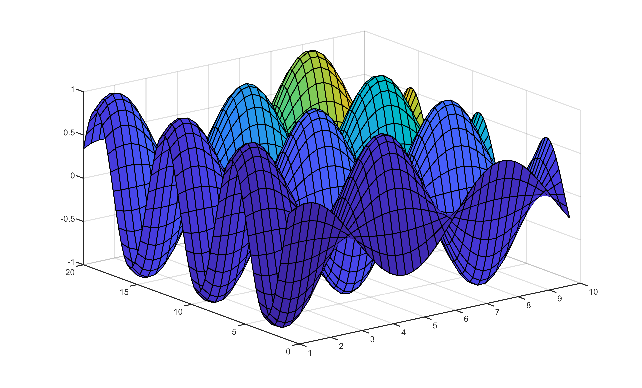
\includegraphics[scale=0.85]{FIG002} 
  \caption{A plot of \(f(x,y)=\sin(x)\cos(y)\).} 
  \end{figure} 
  \begin{figure}[H] 
  \centering 
  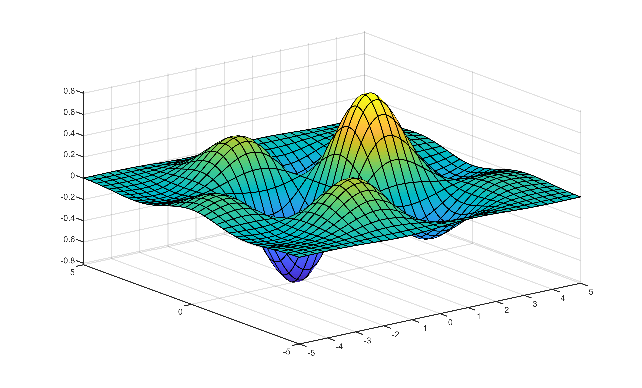
\includegraphics[scale=0.85]{FIG003} 
  \caption{A plot of \(f(x,y)=\sin(x)\cos(y) e^{-\frac{x^2+y^2}{10}}\).} 
  \end{figure} 
  \end{enumerate} 
  
  \section{Postscript} 
  My motivation for writing \textsf{MatLaTex} was the need for a simple system to create problem sets and exams  
  (and answers!) for my math classes. I have been using several computer algebra systems:  
  the symbolic math toolboxes of \textsf{Matlab} and \textsf{Octave}, \textsf{Maple}, \textsf{SageMath}, \textsf{SymPy} and so on. 
  Not wanting to reinvent the wheel I looked at what was available. I started with \textsf{SageTex}; alas, I was 
  never able to properly install and run it. I tried several additional packages and I found each one either  
  too confusing to set up, or not providing the functionalities I wanted, or both. 
   
  Consequently I decided to write my own package. I am a simple guy and \textsf{MatLaTex} is a simple hack.  
  I am certain that any sufficiently interested serious programmer can produce a much better version 
  and I will be very happy if someone does.  
  In the meantime, \textsf{MatLaTex} works  right out of the box and does what I want it to do:  
  programmatically incorporate symbolic and numeric \textsf{Matlab} results into my \LaTeX\  documents.  
   
  In conclusion, there are a few improvements / extensions on which I hope to work in the future. I list them  
  in order of decreasing priority.  
  \begin{enumerate} 
  \item In the current implementation, variable names cannot be ``reused''. If a variable \texttt{a} appears several times 
  in the \LaTeX\ commands, it will always be replaced by its last computed value. I would like to be able 
  to replace each occurrence of \texttt{a} with its value as computed just before this appearance. 
  \item Double matrices should be handled better. 
  \end{enumerate} 
  \noindent Finally, let me mention that I am also working on \textsf{OctLatex} and \textsf{MapleLatex} which are  
  \textsf{Octave} and \textsf{Maple} versions of the \textsf{MatLatex} idea. 
  
  \end{document}